\documentclass[conference]{IEEEtran}
\IEEEoverridecommandlockouts
% The preceding line is only needed to identify funding in the first footnote. If that is unneeded, please comment it out.
\usepackage{cite}
\usepackage{amsmath,amssymb,amsfonts}
\usepackage{algorithmic}
\usepackage{graphicx}
\usepackage{textcomp}
\usepackage{xcolor}
% ACG added
\usepackage{tabulary}
%\usepackage{tabularx}

% ACG added for equation support
\usepackage{amsmath}

% Comment out chunks of text
\usepackage{comment}

% Sub figures
\usepackage{caption}
\usepackage{subcaption}

% ACG
%\usepackage[breaklinks]{hyperref}

% ACG added fmtcount for superscript support, e.g., \ordinalnum{18} = 18^th
\usepackage{fmtcount}

% ACG added hhline for double line support
\usepackage{hhline}

% ACG added for sweet tildes
\newcommand{\mytilde}{\raise.17ex\hbox{$\scriptstyle\mathtt{\sim}$}}

% ACG added for special chars in verbatim
\usepackage{alltt}

% ACG added for float figures
\usepackage{fixltx2e}

% ACG added for float barrier
\usepackage{placeins}

% ACG added for strikeout
\usepackage[normalem]{ulem}

%ACG added for color comments
\usepackage{xcolor}
%\newcommand{\comment}[1]
%{\par {\bfseries \color{blue} #1 \par}} %comment showed

%ACG revised for rebutal
\newcommand{\revise}[1]
{{\color{blue} #1}}

%ACG added for RED
\newcommand{\RED}[1]
{{\bfseries \color{red} #1}}

% ACG copied from ACM
\newcommand{\quotes}[1]{``#1''}
% \newcommand{\note}[1]{{\textcolor{red}{*** NOTE: #1 ***}}}

% ACG added for verbatim that breaks lines and supports color
\usepackage{listings}
%\lstset{basicstyle=\ttfamily,
%  breaklines=true}
\lstnewenvironment{telAPI}[1][]
   {\lstset{basicstyle=\ttfamily\small,
       breaklines=true,
       escapeinside={<@}{@>},
       linewidth=\linewidth, #1}}
   {}

% ACG added for sidewaystable
%\usepackage{rotating}

\usepackage{url}

%SJL added:
\usepackage{flushend}

% remember to use as \metricset{} if you want the space afterward
% definitions
\newcommand{\metricset}{\emph{metric set}}
\newcommand{\streams}{\emph{LDMS Streams}}
\newcommand{\aggregator}{\emph{aggregator}}
\newcommand{\sampler}{\emph{sampler}}
\newcommand{\store}{\emph{store}}
\newcommand{\plugin}{\emph{plugin}}
\newcommand{\plugins}{\emph{plugins}}
\newcommand{\connector}{\emph{Darshan-LDMS Connector}}
\newcommand{\dsampler}{\emph{Darshan Sampler}}
\newcommand{\kernel}{\emph{kernel}}
\newcommand{\kernels}{\emph{kernels}}
\newcommand{\DSOS}{\emph{DSOS}}
\newcommand{\SOS}{\emph{SOS}}
\newcommand{\Darshan}{\emph{Darshan LDMS Integration}}
\newcommand{\appdat}{\emph{application data}}
\newcommand{\AOPP}{\emph{AOPP}}
% Global counter to ID notes/todo macros easily
% Named notes, per person, in color, with a global counter to ID them esily
\newcount\notenum
\notenum=0
\newcommand{\fslnote}[3]        {\global\advance\notenum by 1\textsl{\bf\color{#2}[#1\the\notenum: #3]}}
\newcommand{\todo}[1]{\fslnote{TODO}{red}{#1}}

\def\BibTeX{{\rm B\kern-.05em{\sc i\kern-.025em b}\kern-.08em
    T\kern-.1667em\lower.7ex\hbox{E}\kern-.125emX}}
\begin{document}

\title{LDMS Darshan Connector: Integrating LDMS Streams for run Time Diagnosis of HPC Application I/O Performance}

\author{\IEEEauthorblockN{1\textsuperscript{st} Sara Walton}
\IEEEauthorblockA{\textit{Sandia National Laboratories (of Aff.)} \\
\textit{name of organization (of Aff.)}\\
City, Country \\
email address or ORCID}
}
\begin{comment}
\and
\IEEEauthorblockN{2\textsuperscript{nd} Given Name Surname}
\IEEEauthorblockA{\textit{dept. name of organization (of Aff.)} \\
\textit{name of organization (of Aff.)}\\
City, Country \\
email address or ORCID}
\and
\IEEEauthorblockN{3\textsuperscript{rd} Given Name Surname}
\IEEEauthorblockA{\textit{dept. name of organization (of Aff.)} \\
\textit{name of organization (of Aff.)}\\
City, Country \\
email address or ORCID}
\and
\IEEEauthorblockN{4\textsuperscript{th} Given Name Surname}
\IEEEauthorblockA{\textit{dept. name of organization (of Aff.)} \\
\textit{name of organization (of Aff.)}\\
City, Country \\
email address or ORCID}
\and
\IEEEauthorblockN{5\textsuperscript{th} Given Name Surname}
\IEEEauthorblockA{\textit{dept. name of organization (of Aff.)} \\
\textit{name of organization (of Aff.)}\\
City, Country \\
email address or ORCID}
\and
\IEEEauthorblockN{6\textsuperscript{th} Given Name Surname}
\IEEEauthorblockA{\textit{dept. name of organization (of Aff.)} \\
\textit{name of organization (of Aff.)}\\
City, Country \\
email address or ORCID}
\end{comment}

\maketitle

\begin{abstract}
\RED{ Might need to redo this later}
Improving I/O performance usually depends on a large number of components such as the applications access pattern, the computing system architecture, I/O libraries, file system, mode of access, data size, and the storage configuration and layout. Changes in these components can create high variations in I/O performance which could lead to many negative effects such as network congestion, poor scheduling and indicates a lack of understanding I/O variability. It also makes it difficult to detect the root cause of variations in I/O performance 
%and most of the time strong correlations of I/O analyses across different applications are required to identify a possible solution. 
This paper introduces a unique methodology that provides low latency monitoring of I/O performance variations during run time. This is done through the implementation of a system-level infrastructure that continuously collects I/O application data from an existing I/O characterization tool. This allows insights into the I/O application performance and the components affecting it through the analyses and visualizations.
This methodology addresses the challenge of poor understanding of throughput for system-specific behaviors and variations of I/O performance of similar applications across a system. This paper demonstrates the implementation and assessments of this method and how it can be used on various HPC applications.
\end{abstract}

\section{Introduction}
As more scientific applications are developed and used, the need for improved fidelity and throughput is more pressing than ever and much design effort and investments are being put into improving not only the application but also the system components. Being able to identify, predict and analyze I/O behaviors are critical to ensuring parallel storage systems are utilized efficiently. However, I/O performance continues to show high variations on large-scale production conditions in many cases \RED{Cite NE}. Some of these cases include running applications on clusters during the weekend, separate and disjoint time zones and read I/O's of runs within the same cluster. 
This variation makes it difficult to determine the root cause of I/O related problems and have a thorough understanding of throughput for system-specific behaviors and I/O performance in similar applications across a system. Further, not knowing what the cause is will directly affect the user and developer as unwanted time, effort and investment will need to be put into solving the issue.

Variations in I/O can could be caused by the system behavior such as the file system (e.g. buffering, file transfer, interrupt handling), network congestion, system resource contentions, or the access patterns of the application itself.

Generally, the I/O performance is analyzed post-run by application developers, researchers and users in the form of regression testing or other I/O characterization tools that capture the applications I/O behavior. An example of one of these tools is \emph{Darshan} which captures I/O information on access patterns from HPC applications. Detailed information will be covered in the \emph{Approach} section. In the case where an I/O performance problems are observed, efforts to identify this usually come from any identified correlation between analyses of various applications or the time in which these applications were tested. However, this approach does provide the ability to know \emph{when} an I/O performance variability occurs during an application run and, if the developer or user wishes to, identify any correlations between the file system, network congestion or resource contentions and the I/O performance.

%However, this analysis approach does not take into account the file system, network congestion, system resource contentions and other component's affect on the I/O performance. In order to make these associations, the \emph{absolute timestamps} is required  which the post-run approach and I/O characterization tools usually lack.

The \emph{absolute timestamps} provides run time (e.g. timeseries) data that users and developers could use to better understand how these changing components affect the I/O performance variation as well as provide further insight into the application I/O pattern.This paper will be structured in the following format with the main key factors being:
\begin{itemize}
    \item Describe the approach used to expose absolute timestamp data from an existing I/O characterization tool and utilizing this data to help identify and better understand any root cause(s) of application I/O performance variation run time.
    \item Provide a high level overview of the implementation process and other tools used to collect application I/O data during run time.
    \item Demonstrate use cases of the \connector for various applications on a production HPC system. 
    \item How this new approach provides the ability to collect and assist in the detection of application I/O performance variances across multiple applications. 
\end{itemize}

\section{Related Work}
\RED{Look for papers that used a similar approach}

\section{Approach}

%Therefore, this paper provides an existing system level system
This section provides a high-level overview of the design and implementation of the \Darshan and the components used to create this infrastructure. This approach will provide run time insights about application I/O by using the following tools:
\begin{enumerate}
    \item The I/O characterization tool, Darshan \RED{cite} to collect application I/O behavior and patterns. However, this tool does not report the \emph{absolute timestamp} so modifications to the code were made to expose this data.
    \item The Lightweight Distributed Metric Service (LDMS) \RED{cite} to provide and transport live run time data feed about application I/O events.
    \item A storage database, Distributed Scalable Object Store (DSOS) \RED{cite} to store and query large amounts of data generated on a production HPC system.
    \item An analysis and visualization infrastructure, HPC Web Services \RED{cite}, that use Grafana \RED{cite} and python analysis modules to present run time I/O data. The timeseries data will enable the user to identify when a variability occurs as well as create new meaninful analyses.
\end{enumerate}

Darshan is used to tune applications for increased scientific productivity or performance and is suitable for full time deployment for workload characterization of large systems. It provides detailed statistics about various level file accesses made by MPI and non-MPI applications which can be enabled or disabled as desired. These levels include POSIX, STDIO, LUSTRE and MDHIM for non-MPI applications and MPI-IO, HDF5 and some PnetCDF for MPI applications. This functionality provides users with a summary of I/O behavior and patterns from an application run but it does so post-run. Therefore, it does not allow insights into \emph{run time} I/O behavior and patterns which makes it nearly impossible to identify the root cause(s) of I/O variability and when this occurs. 

LDMS is used to efficiently collect and transport scalable \emph{synchronous} and \emph{event-based} data with low-overhead. Two key functionalities it has that will be leveraged in the \Darshan and create the \connector are the \emph{LDMS Streams} and transport. In the \Darshan, the LDMS was enhanced to support application I/O data injection and store to DSOS while Darshan was modified to expose the \emph{absolute timestamp} and publish run time I/O events for each rank to the \emph{LDMS Streams}. This integration will be described in detail later on.   

%Implementing LDMS into Darshan will provide timestamped I/O event data during an application run. This data will provide any users, application developers or researchers to further their analyses, better understand when an I/O variability occurs and can identify any correlations between the I/O performance and file system, network congestion or system contention.  

\emph{DSOS} will enable the ability to query the timestamped application I/O data through a variety of APIs while Grafana will provide a front-end interface for visualizing the stored data that has been queried and analyzed using Python based modules on the back-end. With these tools, users can view, edit and share analyses of the data as well as create new meaningful analyses. 

The implementation of LDMS into Darshan along with the storage, analysis and visualization components that make up this design will provide detailed insights into the I/O behavior and patterns during run time. This insight will allow users and researchers to better understand how application I/O variability correlates with overall system behavior (e.g. file system, network congestion, etc.) how the time of day affects the I/O performance, how the I/O pattern within a run affects the I/O performance of read and write and why the read and write I/O performance patterns are different and independent of each other. Further, the occurrence of any I/O variabilty can be identified during run time.

%\RED{\begin{itemize}
%    \item Address current I/O performance analysis and implications.
%    \subitem Lesson Learned: Different applications experience high and low performance variations at separate and disjoint time periods.These times periods are shared across different applications and clusters. 
%    \subitem How LDMS will help: It is suggested that a simple I/O monitoring data collection from Darshan will be useful in identifying these time periods. LDMS will be able to provide the run time I/O monitoring data collection which will help them in identifying these time periods. 
%    \subitem Lesson Learned: Clusters running on weekends observe some of the highest performance variations. It is assumed that this could be from I/O intensive application runs during the weekends. 
%    \subitem How LDMS will help: The I/O timeseries data generated by LDMS will provide NERSC researchers with new data they can utilize to further their research.
%    \item Benefits of having time series data:
%    \subitem Better understand how application I/O variability correlates with overall system behavior
%    \subitem Understand how time of day affects the I/O performance
%    \subitem Understand how the I/O pattern within a run affects the I/O performance of read and write. E.g. perhaps an application that has nodes writing data at disjoint times have less I/O performance variation than one that has all nodes writing data at the same time.
%    \subitem Understand why read and write I/O performance patterns are different and independent of each other. E.g. read and write may exhibit different behavior during the run, which affects the performance of each in unique ways

%\end{itemize}
%}

%\subsection{Darshan and LDMS Overview}
%\RED{ \begin{itemize}
%    \item Explain how Darshan works. What is it, who created it, what does it do %exactly? What areas does it lack? (i.e. no timestamps)
%    \item Explain how LDMS works (high level overview -- same as Darshan). What capabilities does it have that we will be applying to Darshan to transport the data.
%    \item Explain how SOS works and why we are using it.
%    \item Explain how Grafana works with SOS and why we are using it. 
%\end{itemize}
%}
\section{Darshan LDMS Integration}
\subsection{Darshan}
Darshan is divided into two main parts: 1) \emph{darshan-runtime} which contains the instrumentation of the characterization tool. It also produces a single log file a the end of each execution summarizing the I/O access patterns used by the application. 2) \emph{darshan-util} which is intended for analyzing log files produced by darshan-runtime. The \Darshan focuses on the \emph{darshan-runtime} as this is where the source code of I/O event data is recorded by Darshan.

Darshan tracks the start, duration and end time of an application run via the C function \emph{clock\_gettime()} and converts the result into seconds and passes the result to a struct that is then used to report the summary log files. Therefore, in order to retrieve the \emph{absolute timestamp} and include it into the I/O event data during run time, a time struct pointer was added to the function call that used \emph{clock\_gettime()} in \emph{darshan-runtime}. This pointer was passed through all of Darshan's modules and the \emph{absolute timestamp} was collected. This was the preferred method as it required minimal changes to Darshan's source code and no additional overhead and latency between the function call and recording of the \emph{absolute timestamp}.  

\subsection{LDMS Streams}
The word, \emph{LDMSD}, refers to an LDMS daemon that provides the capability of data collection, transport and storage and their \emph{plugins} determine the functionality of these capabilities. Daemons on the compute nodes run sampler plugins and transport is achieved through multi-hop \emph{aggregation}. LDMS had two levels of aggregator daemons \RED{cite} which can utilize storage plugins to store any sets of data into various formats so long as it's specified beforehand. This can be seen in \RED{add LDMS fig}
\begin{figure}
  \centering
    %\includegraphics[trim=0.2cm 8.5cm 12cm 0cm ,clip,width=0.9\linewidth]{figs/fig_kokkos_ldms.pdf}
    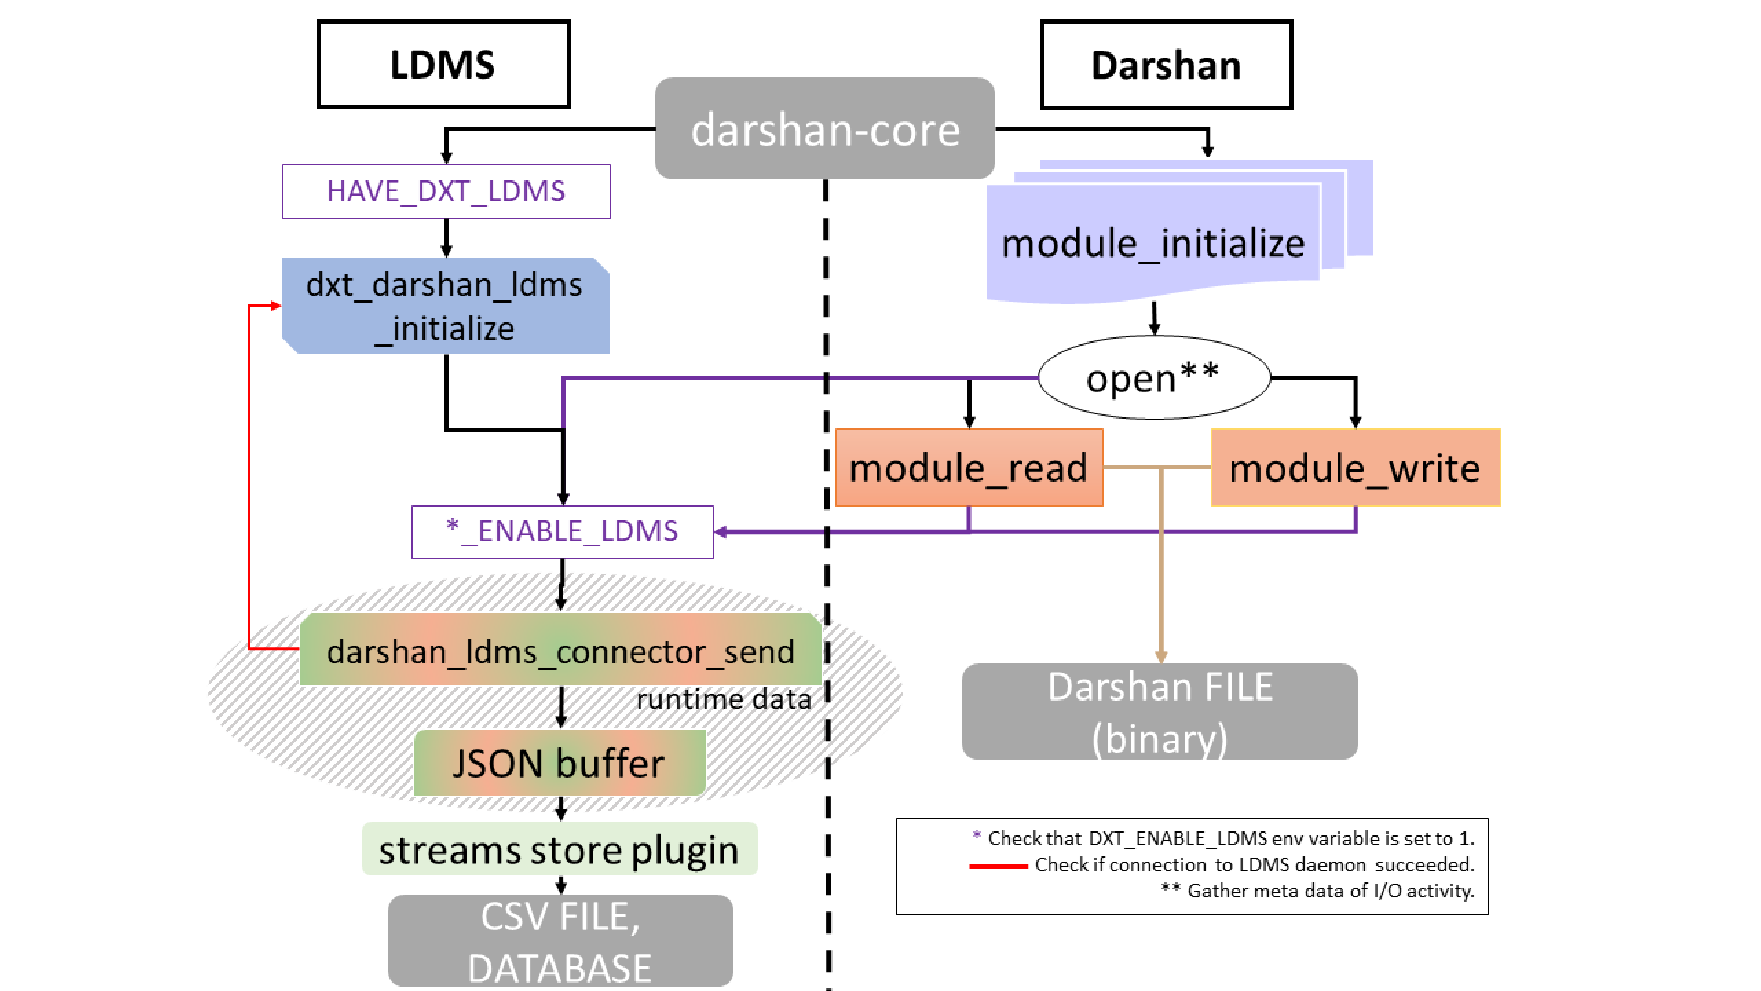
\includegraphics[trim={3.5cm 0 0 0},clip,
    width=1.15\linewidth]{figs/darshan-connector.PNG}
\caption{Overview of the \connector design and how it collects I/O data for each read, write, open and close events per rank from Darshan with little-no interference. The LDMS library must be linked against the Darshan build in order to utilize the \emph{LDMS Streams} functionality and store plugins.}
\label{f:Darshan Connector}
\end{figure}

The \Darshan leverages the LDMS transport to support the injection and transport of application I/O data which requires a \emph{push-based} method to reduce the amount of memory consumed and data loss on the node as well as reduce the latency between the time in which the event occurs and when it is recorded. A \emph{pull-based} method would require a buffering to hold an unknown number of events between pulls. Also, the transported data format needs to support  \emph{variable-length} events because the I/O data may will most likely vary in size. 

This leads to the LDMS \emph{publish-subscribe bus} capability , \emph{LDMS Streams}, which has been enhanced to support I/O event data. This capability is intended for publishing and subscribing to an \emph{LDMS streams tag}. The tag needs to be specified in LDMS daemons and \emph{plugins} in order to publish event data to \emph{LDMS Streams} and receive this published \emph{LDMS Streams} data that match the tag.This process and the \emph{push-based} method can be seen in \RED{figure of LDMS}. Event data can be specified as either \texttt{string} or \texttt{JSON} format. The \emph{LDMS Streams} API was modified to support long application connections and message injections. \emph{LDMS Streams} uses best effort without a reconnect or resend for delivry and does not cache it's data so the published data can only be received after subscription. The \emph{LDMS Streams} allows the ability for any data source to be injected into the LDMS transport.

\subsection{Darshan Connector}

The most recent version of Darshan allows for full tracing of application I/O workloads using their Darshan eXtended Tracing (DXT) instrumentation module which can be enabled and disabled as desired at runtime. This provides high-fidelity traces fo an application's I/O workload vs Darshan's traditional I/O summary data \RED{cite}. DXT currently traces POSIX and MPI-IO layers \RED{cite}. This design leverages the additional I/O tracing Darshan's DXT provides through the new \connector capability.


The \connector functionality collects both DXT data and Darshan's original I/O data and optionally publishes the message in JSON format to the \emph{LDMS Streams} interface. The \emph{absolute timestamp} is also included in this message with the given name "timestamp". The LDMS transport then transports the I/O event data to a \emph{DSOS} database where Grafana can access and query this data. the \connector currently uses a single unique \emph{LDMS Stream tag} for this data source. For the file level accesses that DXT does not trace or for file level access type that have different name-value pairs, a value of "N/A" or "-1" is given in the JSON message in figure \RED{xxx}. 

Depending on the \texttt{"type"} name, the absolute directory of the Darshan file output and executable will be recorded and published to \emph{LDMS Streams}. This decision is based on the \texttt{"type"} name that is set to either \texttt{"MET"}(e.g. "meta") or \texttt{"MOD"}(e.g. "module"). This name is set to "MET" only for open I/O events as this is where Darshan records all I/O data that will not change until the application is complete (e.g. rank, file, node name, etc.). The name is set to "MOD" is for all other I/O events to reduce the message size and latency when sending the data through an HPC production system pipeline.

\begin{figure}
  \centering
    %\includegraphics[trim=0.2cm 8.5cm 12cm 0cm ,clip,width=0.9\linewidth]{figs/fig_kokkos_ldms.pdf}
    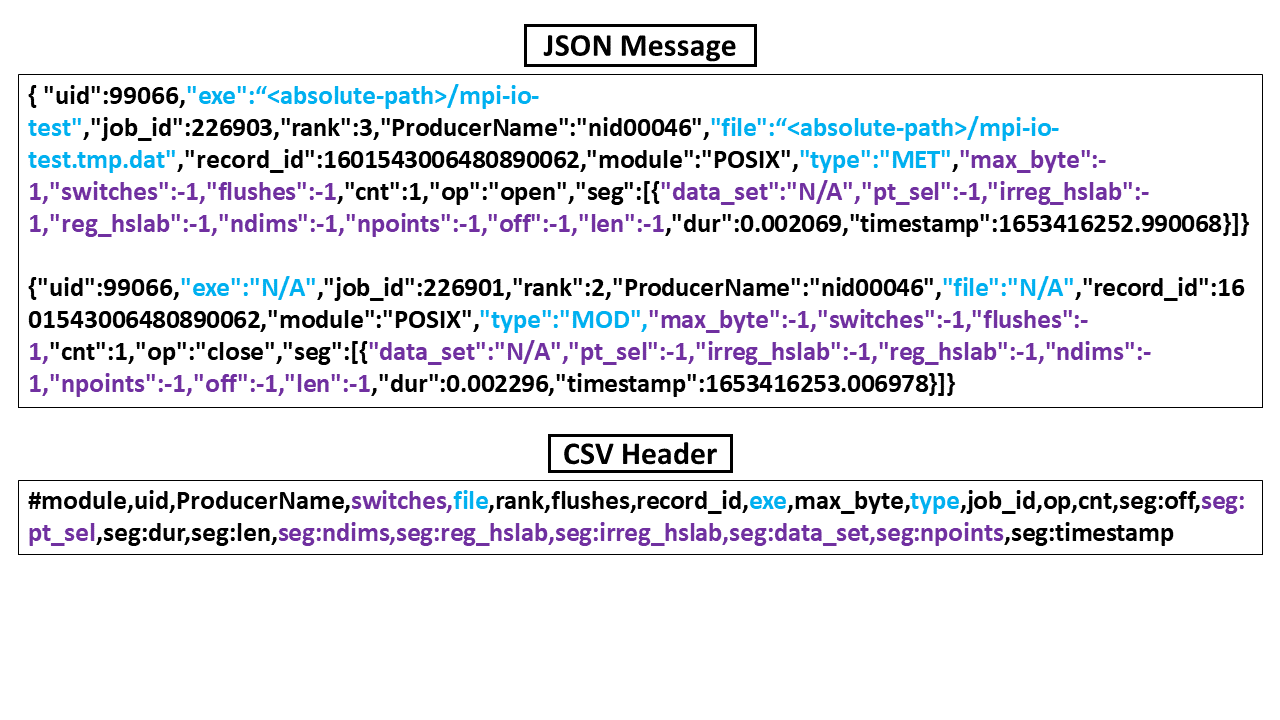
\includegraphics[trim={0 4cm 0 0},clip, width=1\linewidth]{figs/darshan-csv-json.png}
\caption{Output of a simple mpi-io test run. The JSON message is what is being published to the \emph{LDMS Streams} interface that then converts it to CSV and store to \emph{DSOS}. The \texttt{name:value} pairs in light blue indicate meta data stored. while the light purple indicates the data that does not apply to the POSIX file level access and are given the values of "N/A" or "-1".}
\label{f:CSV Header and Output}
\end{figure}

%\section{Additional Components}
%This section will provide a high level overview on how and why the \Darshan approach implemented the DSOS and Grafana tools for storage, analysis and visualization. 
\subsection{Storage: DSOS Database}
DSOS is built on the Scalable Object Store (SOS) database \RED{cite} and was intended to address the domain-specific needs of large-scale HPC monitoring. It was chosen as the preferred database because it allows for interaction via a command line interface which allows for fast query testing and data examination. DSOS also provides scalable data ingest and the ability to query large volumes of data which is required for the large amounts of data to be ingested and stored. %However, a different storage that had similar capabilities could be used instead. 
To sort though the published \emph{LDMS Streams} data, combinations of the job ID, rank and timestamp are used to create joint indices where each index provided a different query performance. An example of this is using \texttt{job\_rank\_time} which will order the data by job, rank then timestamp and then search the data by a specific rank within a specific job over time.

\subsection{Analysis and Visualization: HPC Web Services}
The HPC Web Services \RED{cite} is an infrastructure that consists of the analysis and visualization components of this approach. Any data queries start from a front-end application and transferred to a back-end application that are running on an HPC cluster. In this case the front-end website is Grafana \RED{cite} and the back-end consists of Python analysis modules. The HPC Web Services also provide instant analysis where data can be analyzed and viewed in real time as opposed to the traditional method of querying the results of analyzed data from a separate database.

Grafana is an open-source visualization application that provides various charts, graphs and alerts for supported data sources. It can support multiple data formats but is best suited for timeseries data. It has storage plugins for many database technologies in order to query and render data from multiple data sources. The \Darshan implemented a storage plugin for the DSOS database in order to query this data and visualize it on the Grafana web interface \RED{cite}. 

Python analysis modules are used to produce meaningful visualizations on the queried data from the DSOS database. With these modules, queried data is converted into a pandas dataframe \RED{cite} to allow for easier application of complex calculations, transformations and aggregations on the data. The type of analysis module is specified in the Grafana web interface. This is where the \Darshan will demonstrate how runtime I/O data will provide further insights and understanding into application I/O behavior, patterns, performance variability and any correlations these have with the system behavior.   

%\RED{
%\begin{itemize}
%\item Explain how LDMS is integrated into Darshan. Give an overview on how we implement LDMS Streams into the Darshan DXT section to collect run time I/O data and push to a JSON file that then gets aggregated by LDMS and stored to SOS. Then explain how this stored data is then queried and displayed in a Grafana dashboard.
%\item Add a pic of current Darshan LDMS integration setup (.png) 
%\end{itemize}
%}

\section{Use Cases}\label{AA}
This section provides various use cases of the \Darshan timeseries data that will be used to create new meaningful analyses and insights in the I/O performance variability during an application run.

\RED{Explain the different scenarios we will be testing:
\begin{itemize}
    \item Applications: SWFFT, sw4, sw4lite. Standard baseline: mpi-test. 
    \item Explain what each application does, why it's being tested and how the test was performed (i.e. number of nodes, etc.)
    \item Explain the analysis used to analyze the I/O data and how they provide further insight into the I/O behavior and can allow for correlations between I/O performance and system behavior.
    \item show Grafana graphs, Darshan output (maybe) JSON and any tables (if applicable).
\end{itemize}}


\subsection{Results}
This section covers what significance of the approach to collecting runtime application I/O data and how the new analyses helped provide more insight into I/O behavior.
\RED{
\begin{itemize}
    \item Analyse the results of the use cases
    \item What is the significance of the results?
    \item Throw in a picture of the Grafana Dashboard for each use case
    \item How do these results satisfy and solve the problems described in the the "Problems and Approach" section.
\end{itemize}
}  

\section{Future Work}
This paper covered the \Darshan design and implementation of the \connector which collected I/O data from an I/O characterization tool to create a new timeseries that allows for further insights into I/O behavior and patterns. Five key components were used to develop this design which were the I/O event data (Darshan), data collection (LDMS Streams), storage (DSOS), analysis (Python modules) and visualization (Grafana).
These results of this design proved to enhance both LDMS and Darshan tools as well as create new insights and provide a better understanding to application I/O performance and behavior. 

The next steps are to further expand the \connector and it's capabilities by including more I/O event data and demonstrating advanced insights into correlations between I/O performance and system behavior. We hope the \Darshan will be available as an optional "module" plugin in Darshan so their users may use this tool to better understand their applications I/O performance across HPC systems and clusters. 

%\RED{
%\begin{itemize}
%    \item Explain the purpose of the future work.
%    \item What are our plans for this connector? Will we be implementing \emph{LDMS Streams} across other I/O characterization tools, expanding the streams capabilities on Darshan, testing across other applications, etc.?
%\end{itemize}
%}  

\section*{References}

\RED{FIX REFERENCES}
%\bibliographystyle{IEEEtran}
%\bibliography{IEEEabrv,./SNL}


\end{document}

